\chapter{CƠ SỞ LÝ THUYẾT XÂY DỰNG HỆ THỐNG CẢNH BÁO TÉ NGÃ} 
\label{chap:theoretical_basis} % Chapter label for cross-referencing (consistent with Chapter 1)

\section*{} % Chapter introduction (un-numbered section)
% This transition paragraph sets the stage for the chapter, connecting the research goals from Chapter 1 
% with the theoretical background covered in Chapter 2.
Chương trước đã xác định tính cấp thiết của vấn đề té ngã và đề ra mục tiêu nghiên cứu cụ thể. Để làm cơ sở cho việc thiết kế hệ thống, Chương này sẽ cung cấp nền tảng lý thuyết và tổng quan chuyên sâu về các công nghệ cốt lõi liên quan. Nội dung chương sẽ tập trung phân tích các phương pháp phát hiện té ngã truyền thống và hiện đại, đồng thời đặt nền móng cho các nguyên tắc kỹ thuật (thị giác máy tính, xử lý tín hiệu và phần cứng nhúng) được áp dụng trong luận văn.

% --- START OF CHAPTER SECTIONS ---
% The following commands input the individual sections (the 2.x files)
% Ensure these files contain \section{} and \subsection{} commands, not \chapter{}.
\section{Tổng quan về các phương pháp phát hiện té ngã}

% Introducing the importance of fall detection and its global context
Phát hiện té ngã là một lĩnh vực nghiên cứu trọng yếu, đặc biệt trong bối cảnh dân số già hóa đang gia tăng trên toàn cầu. Theo Tổ chức Y tế Thế giới (WHO), té ngã là nguyên nhân đứng thứ hai gây tử vong do thương tích không cố ý trên toàn thế giới, với khoảng 684.000 ca tử vong và hàng triệu ca chấn thương mỗi năm~\cite{who2021}. Các hệ thống phát hiện té ngã tự động không chỉ giúp cảnh báo kịp thời mà còn hỗ trợ cứu sống, giảm thiểu thương tích và cải thiện chất lượng chăm sóc sức khỏe. Các phương pháp hiện nay được phân loại thành bốn nhóm chính: cảm biến đeo được, cảm biến môi trường, thị giác máy tính và kết hợp đa phương thức, mỗi nhóm đều có ưu và nhược điểm riêng biệt.

% Subsection for wearable sensor-based methods
\subsection{Phương pháp dựa trên cảm biến đeo được}

Phương pháp này sử dụng các thiết bị đeo trên cơ thể để thu thập dữ liệu chuyển động, được ứng dụng rộng rãi nhờ tính linh hoạt và chi phí thấp.

\begin{itemize}
    \item \textbf{Cơ chế hoạt động:} Các thiết bị đeo tích hợp cảm biến quán tính như \textbf{gia tốc kế} (đo gia tốc tuyến tính), \textbf{con quay hồi chuyển} (đo tốc độ góc) và đôi khi \textbf{từ kế} (đo định hướng). Dữ liệu được phân tích thời gian thực để phát hiện các mẫu chuyển động bất thường. Một sự kiện té ngã thường được xác định khi gia tốc vượt ngưỡng (ví dụ: 3g) hoặc khi chuyển động đột ngột dừng lại, theo sau là trạng thái bất động~\cite{xu2023}. Các thuật toán phổ biến bao gồm ngưỡng tĩnh (static thresholding), học máy (SVM, Decision Tree) và học sâu (LSTM, CNN). Ví dụ, Hussain và cộng sự~\cite{hussain2019} sử dụng MPU6050 với LSTM, đạt độ chính xác 94.1\% trên tập dữ liệu SisFall.
    \item \textbf{Ưu điểm:} 
    \begin{itemize}
        \item Độ chính xác cao trong việc ghi nhận dữ liệu chuyển động cá nhân.
        \item Phản hồi nhanh, phù hợp với giám sát thời gian thực.
        \item Hoạt động độc lập với điều kiện môi trường như ánh sáng hay cấu trúc không gian.
        \item Chi phí thấp với các thiết bị như đồng hồ thông minh hoặc vòng đeo tay~\cite{wearable20152024}.
    \end{itemize}
    \item \textbf{Nhược điểm:}
    \begin{itemize}
        \item Yêu cầu người dùng đeo thiết bị liên tục, gây bất tiện hoặc dễ bị quên, đặc biệt với người cao tuổi.
        \item Dễ gây cảnh báo sai khi thực hiện các hoạt động mạnh như chạy, nhảy hoặc ngồi xuống nhanh, với tỷ lệ false positive có thể lên đến 20\%~\cite{alarifi2021}.
        \item Pin và hiệu chuẩn định kỳ là vấn đề, đặc biệt với các cảm biến cần bảo trì thường xuyên.
    \end{itemize}
\end{itemize}

% Subsection for environment-based sensor methods
\subsection{Phương pháp dựa trên cảm biến môi trường}

Phương pháp này sử dụng các cảm biến cố định trong không gian sống, phù hợp cho giám sát tại nhà hoặc cơ sở y tế mà không cần người dùng đeo thiết bị.

\begin{itemize}
    \item \textbf{Cơ chế hoạt động:} Các cảm biến phổ biến bao gồm \textbf{cảm biến áp suất sàn} (phát hiện thay đổi trọng lượng), \textbf{cảm biến hồng ngoại thụ động (PIR)} (phát hiện chuyển động hoặc bất động) và \textbf{cảm biến âm thanh} (nhận diện tiếng va chạm). Ví dụ, cảm biến áp suất sàn phát hiện sự thay đổi trọng lượng bất thường (ví dụ: từ 60 kg xuống 0 kg trong 0.5 giây), trong khi cảm biến PIR ghi nhận sự bất động kéo dài~\cite{smartfloor2024}. Các hệ thống hiện đại tích hợp AI để phân tích dữ liệu, như mô hình học sâu trên cảm biến âm thanh đạt độ chính xác 92\% trong môi trường thử nghiệm~\cite{chen2024}. 
    \item \textbf{Ưu điểm:} 
    \begin{itemize}
        \item Không xâm phạm, không yêu cầu người dùng đeo thiết bị, phù hợp với người cao tuổi không muốn sử dụng thiết bị cá nhân.
        \item Có thể giám sát nhiều người trong một khu vực, lý tưởng cho nhà dưỡng lão hoặc bệnh viện.
        \item Dễ tích hợp vào hệ thống nhà thông minh (smart home).
    \end{itemize}
    \item \textbf{Nhược điểm:}
    \begin{itemize}
        \item Chi phí lắp đặt cao, đặc biệt với cảm biến sàn, có thể lên đến hàng nghìn USD cho một căn hộ~\cite{smartfloor2024}.
        \item Phạm vi giám sát giới hạn, dẫn đến "điểm mù" ở các khu vực không có cảm biến.
        \item Khó phân biệt giữa người và vật thể (ví dụ: vật nuôi, đồ vật rơi), gây cảnh báo sai với tỷ lệ lên đến 15\% trong môi trường phức tạp~\cite{chen2024}.
    \end{itemize}
\end{itemize}

% Subsection for vision-based methods
\subsection{Phương pháp dựa trên thị giác máy tính}

Phương pháp này sử dụng camera và thuật toán xử lý ảnh để phân tích tư thế và chuyển động, mang lại thông tin trực quan phong phú mà không cần tiếp xúc vật lý.

\begin{itemize}
    \item \textbf{Cơ chế hoạt động:} Hệ thống sử dụng camera RGB, camera độ sâu (RGB-D) hoặc camera hồng ngoại để thu thập video. Các bước xử lý bao gồm: (1) phát hiện con người bằng mô hình như YOLOv5/v8, (2) ước tính tư thế với các framework như OpenPose, MediaPipe hoặc MoveNet, trích xuất các điểm khớp xương (keypoints), và (3) phân tích động học keypoints để xác định té ngã (ví dụ: chuyển từ tư thế đứng sang nằm trong dưới 1 giây). Ví dụ, Bugarin và cộng sự~\cite{bugarin2022} sử dụng MediaPipe đạt F1-score 91.4\% trên tập dữ liệu MCFD. Các mô hình học sâu như Transformer hoặc CNN-LSTM được áp dụng để cải thiện độ chính xác, đạt mAP 98.6\% trong một số nghiên cứu~\cite{han2024}.
    \item \textbf{Ưu điểm:} 
    \begin{itemize}
        \item Cung cấp thông tin bối cảnh trực quan, hỗ trợ xác nhận sự cố dễ dàng hơn thông qua hình ảnh hoặc video.
        \item Không yêu cầu người dùng đeo thiết bị, giảm bất tiện và tăng chấp nhận từ người dùng.
        \item Có thể tích hợp với hệ thống giám sát an ninh hiện có.
    \end{itemize}
    \item \textbf{Nhược điểm:}
    \begin{itemize}
        \item Lo ngại về quyền riêng tư, đặc biệt khi sử dụng camera trong không gian riêng như phòng ngủ hoặc phòng tắm.
        \item Hiệu suất phụ thuộc vào ánh sáng, góc quay và sự che khuất, với độ chính xác giảm 10--20\% trong điều kiện ánh sáng yếu~\cite{saraswat2024}.
        \item Yêu cầu phần cứng tính toán mạnh, đặc biệt với các mô hình học sâu như Transformer, gây khó khăn cho triển khai trên thiết bị biên~\cite{stylios2024}.
    \end{itemize}
\end{itemize}

% Subsection for multi-modal methods
\subsection{Phương pháp kết hợp đa phương thức}

Phương pháp này kết hợp nhiều nguồn dữ liệu để cải thiện độ chính xác và độ tin cậy, tận dụng ưu điểm của các phương pháp riêng lẻ.

\begin{itemize}
    \item \textbf{Cơ chế hoạt động:} Hệ thống tích hợp dữ liệu từ cảm biến đeo (IMU), camera (RGB hoặc RGB-D), và đôi khi cảm biến môi trường. Các thuật toán \textbf{sensor fusion} (như Kalman Filter hoặc học sâu) kết hợp dữ liệu để đưa ra quyết định. Ví dụ, một sự kiện té ngã được xác nhận khi cảm biến IMU ghi nhận gia tốc bất thường và camera phát hiện tư thế nằm ngang~\cite{rougier2011}. Keskes và Noumeir~\cite{keskes2021} sử dụng mạng ST-GCN để xử lý đồng thời dữ liệu skeleton từ OpenPose và tín hiệu IMU, đạt F1-score 93.2\%. Các nghiên cứu gần đây (2024) tích hợp thêm cảm biến mmWave (như MR60FDA2) để tăng độ chính xác lên 95\% trong môi trường phức tạp~\cite{mmwave2025}.
    \item \textbf{Ưu điểm:} 
    \begin{itemize}
        \item Giảm đáng kể tỷ lệ cảnh báo sai (xuống dưới 5\% trong một số hệ thống) nhờ xác minh đa nguồn~\cite{multimodal2024}.
        \item Mở rộng phạm vi giám sát, phù hợp cho cả trong nhà và ngoài trời.
        \item Tăng tính linh hoạt, có thể tùy chỉnh theo môi trường và nhu cầu cụ thể.
    \end{itemize}
    \item \textbf{Nhược điểm:}
    \begin{itemize}
        \item Độ phức tạp cao, yêu cầu thuật toán và phần cứng xử lý mạnh, tăng chi phí triển khai.
        \item Tiêu thụ năng lượng lớn, đặc biệt khi tích hợp nhiều cảm biến và camera.
        \item Khó khăn trong việc đồng bộ dữ liệu từ các nguồn khác nhau, có thể gây độ trễ trong xử lý thời gian thực~\cite{liu2018}.
    \end{itemize}
\end{itemize}

\subsection{Lợi thế của phương pháp tiếp cận đa phương thức}
Các phương pháp phát hiện té ngã dựa trên một nguồn dữ liệu duy nhất (chẳng hạn như chỉ cảm biến quán tính hoặc chỉ thị giác máy tính) thường đối mặt với những hạn chế về độ chính xác và khả năng ứng dụng trong các bối cảnh đa dạng \cite{researchgate_hybrid}. Để khắc phục những điểm yếu này, hệ thống của đề tài đã phát triển một phương pháp tiếp cận đa phương thức (multi-modal) độc đáo, tích hợp và tận dụng thế mạnh của cả hai công nghệ, mang lại nhiều lợi ích vượt trội.

\subsubsection{Cải thiện độ chính xác và giảm cảnh báo sai thông qua kết hợp dữ liệu}
Một trong những thách thức lớn nhất của các hệ thống phát hiện té ngã là tỷ lệ cảnh báo sai (false positive rate) cao. Phương pháp tiếp cận đa phương thức giải quyết vấn đề này bằng cách sử dụng cơ chế \textbf{kết hợp dữ liệu (data fusion)} ở cấp độ quyết định, một kỹ thuật đã được chứng minh là tăng cường độ tin cậy của hệ thống \cite{mdpi_data_fusion}. Cụ thể, một sự kiện chỉ được xác nhận là té ngã khi cả hai hệ thống con đưa ra kết luận độc lập và khớp với nhau:

\begin{itemize}
    \item \textbf{Phát hiện từ cảm biến quán tính (IMU):} Thiết bị đeo trên người, tích hợp cảm biến gia tốc và con quay hồi chuyển, phân tích các thay đổi đột ngột về gia tốc tuyến tính và tốc độ góc \cite{resna_imu}. Thuật toán sẽ kích hoạt khi gia tốc vượt ngưỡng xác định, theo sau là một trạng thái bất động kéo dài (post-fall inactivity).
    \item \textbf{Phát hiện từ thị giác máy tính:} Máy chủ cục bộ xử lý luồng video từ camera, sử dụng các thuật toán ước tính tư thế (pose estimation) tiên tiến để xác định vị trí các khớp xương. Một mô hình logic sẽ nhận diện sự thay đổi tư thế đột ngột từ đứng thẳng sang nằm ngang, được biểu thị bằng tỷ lệ giữa chiều cao và chiều rộng cơ thể giảm xuống dưới một ngưỡng nhất định.
\end{itemize}

Bảng \ref{tab:so_sanh_phuong_phap} dưới đây minh họa rõ ràng ưu điểm của cơ chế kết hợp dữ liệu so với các phương pháp đơn lẻ.

\begin{table}[h!]
    \centering
    \caption{So sánh các phương pháp phát hiện té ngã}
    \label{tab:so_sanh_phuong_phap}
    \begin{tabular}{|p{0.25\linewidth}|p{0.3\linewidth}|p{0.3\linewidth}|}
        \hline
        \textbf{Kịch bản} & \textbf{Hệ thống đơn lẻ} & \textbf{Hệ thống đa phương thức} \\
        \hline
        Người dùng ngồi nhanh xuống ghế & Có khả năng cảnh báo sai do thay đổi gia tốc và tư thế đột ngột. & Không cảnh báo vì tư thế "nằm" trên sàn không được xác nhận. \\
        \hline
        Người dùng té ngã thật sự & Cả hai hệ thống đều có thể đưa ra cảnh báo chính xác. & Cảnh báo chỉ được kích hoạt khi cả hai tín hiệu xác nhận (thay đổi gia tốc/tư thế và trạng thái nằm ngang). \\
        \hline
        Người dùng té ngã ngoài tầm camera & Không thể phát hiện té ngã. & Vẫn phát hiện nhờ cảm biến IMU trên thiết bị đeo. \\
        \hline
    \end{tabular}
\end{table}

\subsubsection{Mở rộng phạm vi giám sát và tính linh hoạt}
Một trong những ưu điểm cốt lõi của phương pháp đa phương thức là khả năng mở rộng phạm vi giám sát, vượt qua các hạn chế vật lý của các giải pháp truyền thống. Hệ thống có khả năng chuyển đổi linh hoạt giữa hai chế độ hoạt động:

\begin{itemize}
    \item \textbf{Chế độ giám sát tại chỗ (In-situ Monitoring):} Khi người dùng ở trong tầm bao phủ của camera, hệ thống hoạt động ở chế độ này. Dữ liệu video được xử lý cục bộ trên máy chủ (on-premise processing), đảm bảo quyền riêng tư và tận dụng được sức mạnh tính toán của các mô hình học sâu.
    \item \textbf{Chế độ giám sát di động (Mobile Monitoring):} Khi người dùng di chuyển ra khỏi tầm nhìn của camera, hệ thống tự động chuyển sang chế độ di động. Thiết bị đeo sử dụng \textbf{xử lý tại thiết bị (edge computing)} để phân tích dữ liệu cảm biến và gửi cảnh báo cùng tọa độ vị trí qua mạng di động, đảm bảo an toàn không bị gián đoạn và giải quyết triệt để bài toán "điểm mù" của camera \cite{researchgate_edge_computing}.
\end{itemize}

\subsubsection{Tính ổn định, kinh tế và hiệu quả triển khai}
Việc tích hợp các công nghệ mã nguồn mở và kiến trúc module mang lại một giải pháp ổn định, kinh tế và dễ dàng triển khai.

\begin{itemize}
    \item \textbf{Tính dự phòng trong truyền thông:} Hệ thống được thiết kế với hai kênh truyền thông độc lập. Kênh mạng nội bộ (LAN) sử dụng giao thức \textbf{SIP} để gọi điện khẩn cấp, hoạt động độc lập với Internet. Kênh Internet sử dụng giao thức \textbf{MQTT} nhẹ và hiệu quả, lý tưởng cho việc giám sát từ xa trong môi trường IoT \cite{parangat_mqtt}. Sự kết hợp này đảm bảo cảnh báo luôn được gửi đi ngay cả khi một trong hai kênh gặp sự cố.
    \item \textbf{Hiệu quả kinh tế:} Bằng cách sử dụng các linh kiện nhúng giá thành thấp và các nền tảng phần mềm mã nguồn mở, tổng chi phí đầu tư ban đầu thấp hơn đáng kể so với các giải pháp thương mại, làm tăng tính khả thi của dự án.
    \item \textbf{Khả năng mở rộng (Scalability):} Kiến trúc module cho phép dễ dàng mở rộng hệ thống bằng cách thêm các thiết bị camera và cảm biến mới, phù hợp cho việc triển khai tại các cơ sở y tế hoặc viện dưỡng lão.
\end{itemize}

\subsection{Bảo mật và quyền riêng tư}
Vấn đề bảo mật và quyền riêng tư là ưu tiên hàng đầu, đặc biệt với các hệ thống sử dụng camera. Hệ thống đã giải quyết vấn đề này thông qua các cơ chế sau:
\begin{itemize}
    \item \textbf{Xử lý cục bộ (On-premise Processing):} Dữ liệu video thô được xử lý trên máy chủ cục bộ và không bao giờ được truyền ra Internet, giảm thiểu tối đa nguy cơ bị lộ lọt.
    \item \textbf{Dữ liệu tối thiểu:} Chỉ các thông tin đã được xử lý (như sự kiện té ngã và tọa độ) được gửi đi.
    \item \textbf{Tùy chọn linh hoạt:} Hệ thống có thể được cấu hình để chỉ sử dụng cảm biến ở những khu vực nhạy cảm về quyền riêng tư như khu vực vệ sinh và sinh hoạt cá nhân.
\end{itemize}

\section{Các Giao Thức Truyền Thông}
\label{sec:communication_protocols}
Tiếp nối các phân tích về tình hình nghiên cứu hiện có và các khoảng trống công nghệ được xác định trong phần tổng quan và tình hình nghiên cứu. Chương này chuyển trọng tâm sang trình bày chi tiết về các \textbf{cơ sở lý thuyết và giao thức nền tảng} chi phối hoạt động của Hệ thống Cảnh báo Viễn thông Nhúng IoT được đề xuất, đặc biệt trong ứng dụng \textbf{Phát hiện Ngã (Fall Detection)}.

Trong hệ thống cảnh báo thời gian thực, nơi tính kịp thời của thông tin là yếu tố quyết định, khả năng \textbf{giao tiếp không gián đoạn} giữa các thành phần nhúng và trung tâm điều khiển là tối quan trọng. Chương này sẽ hệ thống hóa các giao thức truyền thông cốt lõi. Cụ thể, \textbf{Giao thức Khởi tạo Phiên (SIP)} sẽ được làm rõ như xương sống cho việc truyền tải âm thanh/video cảnh báo theo thời gian thực; \textbf{Message Queuing Telemetry Transport (MQTT)} được phân tích như một giải pháp \textit{lightweight} và hiệu quả để vận chuyển dữ liệu cảm biến (như dữ liệu gia tốc kế, con quay hồi chuyển sau khi xử lý thuật toán phát hiện ngã) trên các mạng bị hạn chế băng thông; và \textbf{JavaScript Object Notation (JSON)} như định dạng chuẩn để cấu trúc và trao đổi thông tin. Việc nắm vững các cơ chế này là nền tảng để xây dựng và đảm bảo hiệu suất của một hệ thống cảnh báo từ xa, tin cậy và có khả năng mở rộng.
\subsection{Giao Thức Khởi Tạo Phiên (SIP)}
\label{subsec:sip_protocol}

SIP là giao thức báo hiệu nền tảng của VoIP, dùng để khởi tạo, quản lý và kết thúc các phiên đa phương tiện qua mạng IP~\cite{sip_rfc3261}. SIP hỗ trợ gọi thoại, hội nghị video, nhắn tin tức thời và thông tin hiện diện. Nó hoạt động ở lớp ứng dụng của mô hình TCP/IP, sử dụng các phương thức dựa trên văn bản tương tự HTTP để đảm bảo tính linh hoạt và dễ mở rộng.

\subsubsection{Kiến Trúc và Luồng Thông Điệp}
\label{subsubsec:sip_architecture}

SIP hoạt động thông qua trao đổi thông điệp giữa \textit{User Agent Clients} (UACs) và \textit{User Agent Servers} (UASs), với sự hỗ trợ của các máy chủ trung gian: \textbf{Proxy Server} (chuyển tiếp tin nhắn), \textbf{Registrar Server} (lưu trữ thông tin đăng ký) và \textbf{Redirect Server} (hướng UAC tới địa chỉ khác). Các thông điệp chính gồm:

\begin{itemize}
\item \textbf{INVITE}: Khởi tạo phiên hoặc cuộc gọi.
\item \textbf{ACK}: Xác nhận phản hồi thành công cho INVITE.
\item \textbf{BYE}: Kết thúc phiên.
\item \textbf{CANCEL}: Hủy yêu cầu đang xử lý.
\item \textbf{REGISTER}: Đăng ký thông tin thiết bị.
\item \textbf{OPTIONS}: Truy vấn khả năng của máy chủ.
\end{itemize}

SIP kết hợp với \textit{Session Description Protocol} (SDP) để định nghĩa tham số phiên (như codec, cổng) và \textit{Real-time Transport Protocol} (RTP) để truyền dữ liệu thoại/video thời gian thực. Ngoài ra, RTCP (RTP Control Protocol) được sử dụng để giám sát chất lượng truyền dẫn.

\subsubsection{Phân biệt Đường tín hiệu và Đường truyền phương tiện}
\label{subsubsec:sip_paths}

Đây là một sự khác biệt quan trọng trong VoIP:

\begin{itemize}
\item \textbf{Đường tín hiệu (Signaling Path):} Mang các tin nhắn SIP (INVITE, BYE, 200 OK, v.v.) để thiết lập, quản lý và kết thúc cuộc gọi. Đường này thường sử dụng TCP (để truyền tải đáng tin cậy, đặc biệt cho các tin nhắn lớn hơn hoặc các kết nối kéo dài) hoặc UDP (để có độ trễ thấp hơn, đặc biệt cho các tin nhắn nhỏ hơn như REGISTER).
\item \textbf{Đường truyền phương tiện (Media Path):} Mang dữ liệu thoại/video thực tế bằng RTP qua UDP. Sau khi cuộc gọi được thiết lập thông qua tín hiệu, phương tiện truyền trực tiếp giữa các điểm cuối (hoặc thông qua một bộ chuyển tiếp phương tiện trung gian như máy chủ TURN hoặc SBC).
\end{itemize}

Dưới đây là sơ đồ minh họa sự khác biệt giữa đường tín hiệu và đường truyền phương tiện:

%-------- figure--------
\begin{figure}[htb!] 
\centering
\begin{tikzpicture}[
    box/.style={rectangle, draw, rounded corners, minimum height=1em, minimum width=3em, align=center, fill=blue!10}, 
    signal_arrow/.style={-Stealth, thick, blue!70!white, shorten >=1pt, shorten <=1pt}, 
    media_arrow/.style={-Stealth, thick, red!70!white, shorten >=1pt, shorten <=1pt}, 
    label_style/.style={font=\small, align=center, text=black},
    node distance=2.5cm and 3.5cm 
]
    % Định nghĩa các Node
    \node[box] (A) {SIP Endpoint A};
    \node[box, right=of A] (Proxy) {SIP Proxy/PBX \\ (Asterisk)}; 
    \node[box, right=of Proxy] (B) {SIP Endpoint B};
    
    % Node cho Media Proxy (nằm dưới Asterisk PBX)
    \node[box, below=2.5cm of Proxy] (MediaProxy) {Asterisk Media Proxy}; 
    
    % Vẽ đường tín hiệu
    \draw[signal_arrow] (A) -- node[above=2pt, label_style] {SIP Signaling \\ (TCP/UDP)} (Proxy);
    \draw[signal_arrow] (Proxy) -- node[above=2pt, label_style] {SIP Signaling \\ (TCP/UDP)} (B);
    
    % Vẽ đường truyền phương tiện
    \draw[media_arrow] (A) -- node[midway, left=2pt, label_style] {RTP Media Path \\ (UDP)} (MediaProxy); 
    \draw[media_arrow] (MediaProxy) -- node[midway, right=2pt, label_style] {RTP Media Path \\ (UDP)} (B); 
\end{tikzpicture}
\caption{Minh họa sự khác biệt giữa đường tín hiệu và đường truyền phương tiện trong VoIP}
\label{fig:sip-media-path-distinction} 
\end{figure}
\subsubsection{SIP trong Hệ Thống Cảnh Báo Asterisk}
\label{subsubsec:sip_asterisk_integration}

Trong hệ thống cảnh báo dựa trên Asterisk, SIP kết nối điện thoại IP, softphone và PBX qua SIP trunk, mang lại lợi ích:

\begin{itemize}
\item \textbf{Quản lý tập trung}: Đồng nhất cấu hình và quản lý thiết bị.
\item \textbf{Tương thích cao}: Hỗ trợ đa dạng nền tảng và thiết bị.
\item \textbf{Chuẩn mở}: Tích hợp dễ dàng với hạ tầng viễn thông hiện có.
\item \textbf{Bảo mật}: Hỗ trợ mã hóa qua \textbf{TLS} (cho kênh SIP) và \textbf{SRTP} (cho luồng RTP) để bảo vệ dữ liệu.
\end{itemize}

Asterisk đóng vai trò như một SIP server, xử lý đăng ký và định tuyến cuộc gọi.

\subsubsection{Luồng Phân Phối Cảnh Báo}
\label{subsubsec:sip_alert_flows}

\paragraph{Đăng ký}
Thiết bị SIP gửi REGISTER tới Asterisk để xác thực và lưu thông tin liên lạc, thường kèm theo thông tin xác thực (username, password) trong header Authorization.

\paragraph{Thiết lập phiên}
Ứng dụng Linux ra lệnh cho Asterisk khởi tạo cuộc gọi qua AMI (lệnh \texttt{Originate}). Asterisk gửi INVITE, nhận phản hồi (180 Ringing, 200 OK) và xác nhận bằng ACK. Có thể dùng header \texttt{Alert-Info: ;info=alert-autoanswer} để tự động trả lời, giúp phân phối cảnh báo nhanh chóng mà không cần tương tác thủ công.

\paragraph{Trao đổi dữ liệu}
Dữ liệu cảnh báo truyền qua RTP. Nếu dùng TTS (Text-to-Speech), Asterisk tạo âm thanh từ văn bản và phát tới người nhận qua các codec như G.711 hoặc G.729.

\paragraph{Kết thúc phiên}
Một bên gửi BYE, bên kia phản hồi 200 OK để đóng phiên an toàn.

\subsubsection{Tích Hợp SMS qua SIP}
\label{subsubsec:sip_sms}

Có thể gửi SMS trong Asterisk bằng cách kích hoạt \texttt{textsupport=yes} trong \texttt{sip.conf} và định nghĩa logic xử lý trong \texttt{extensions.conf}. Ví dụ, sử dụng lệnh \texttt{MessageSend} để gửi tin nhắn SIP MESSAGE, tích hợp với các nhà cung cấp SMS gateway để chuyển tiếp sang mạng di động.

---

\subsection{Giao Thức Message Queuing Telemetry Transport (MQTT)}
\label{subsec:mqtt_protocol}

MQTT là giao thức nhẹ, tối ưu cho truyền thông M2M trong IoT, hoạt động trên TCP/IP với cơ chế kết nối lâu dài~\cite{mqtt_oasis_standard}. Nó được thiết kế cho các thiết bị có tài nguyên hạn chế, băng thông thấp và kết nối không ổn định.

\subsubsection{Kiến Trúc Publish/Subscribe}
\label{subsubsec:mqtt_pubsub}

MQTT dùng mô hình publish/subscribe qua broker trung tâm (như Mosquitto hoặc HiveMQ), mang lại:
\begin{itemize}
\item \textbf{Tách rời không gian}: Không cần biết địa chỉ IP của nhau.
\item \textbf{Tách rời thời gian}: Không yêu cầu kết nối đồng thời, hỗ trợ \textbf{retained messages} (tin nhắn được lưu lại để gửi cho subscriber mới) và \textbf{clean session} (quản lý trạng thái phiên của client).
\item \textbf{Tách rời đồng bộ}: Truyền và nhận độc lập, giảm độ trễ.
\item \textbf{Bảo mật}: Hỗ trợ TLS, xác thực username/password, và ACL để kiểm soát truy cập topic.
\end{itemize}

Các lệnh chính: CONNECT, PUBLISH, SUBSCRIBE, UNSUBSCRIBE, DISCONNECT. Topic sử dụng cấu trúc phân cấp như \texttt{sensor/room/temperature}.

\subsubsection{Mức QoS}
\label{subsubsec:mqtt_qos}

MQTT cung cấp 3 mức QoS để đảm bảo độ tin cậy.

\begin{itemize}
\item \textbf{QoS 0 (At most once)}: Gửi một lần, không xác nhận, phù hợp cho dữ liệu không quan trọng.
\item \textbf{QoS 1 (At least once)}: Gửi ít nhất một lần, có xác nhận (PUBACK), có thể trùng lặp.
\item \textbf{QoS 2 (Exactly once)}: Gửi đúng một lần qua bắt tay bốn bước (PUBREC, PUBREL, PUBCOMP), đảm bảo tin cậy cao.
\end{itemize}

Trong hệ thống IoT, QoS được chọn dựa trên mức độ quan trọng của dữ liệu cảnh báo.

---

\subsection{JavaScript Object Notation (JSON)}
\label{subsec:json_format}

JSON là định dạng dữ liệu nhẹ, dễ đọc, dùng rộng rãi trong IoT và viễn thông để trao đổi dữ liệu có cấu trúc~\cite{json_rfc8259}. Nó dựa trên cú pháp JavaScript nhưng độc lập ngôn ngữ.

\subsubsection{Ứng Dụng JSON}
\label{subsubsec:json_applications}

\begin{itemize}
\item Lưu cấu hình thiết bị và máy chủ.
\item Trao đổi dữ liệu cảm biến, cảnh báo giữa các thành phần hệ thống.
\item Tương thích đa nền tảng, dễ phân tích bằng các thư viện như \textit{json-c} cho C, hoặc \textit{ArduinoJson} cho ESP32.
\item Tối ưu hóa payload cho MQTT và SIP bằng cách giảm độ dài tên khóa và loại bỏ khoảng trắng.
\end{itemize}

\subsubsection{Ví Dụ JSON}
\label{subsubsec:json_examples}

\begin{figure}[H]
\centering
\begin{minted}[frame=single, breaklines, bgcolor=lightgray, xleftmargin=10pt, linenos]{json}
{
  "network": {
    "ssid": "IoT_Network",
    "password": "MatKhauBaoMat123",
    "mqtt_broker": "192.168.1.100",
    "mqtt_port": 1883
  },
  "device": {
    "id": "ESP32_Sensor_01",
    "location": "Tang_May_A"
  }
}
\end{minted}
\caption{Cấu hình ESP32}
\label{fig:json_esp32_config}
\end{figure}

\begin{figure}[H]
\centering
\begin{minted}[frame=single, breaklines, bgcolor=lightgray, xleftmargin=10pt, linenos]{json}
{
  "device_id": "ESP32_Sensor_01",
  "timestamp": "2024-03-15T10:30:00Z",
  "readings": {
    "temperature": {
      "value": 87.5,
      "unit": "celsius",
      "status": "critical"
    }
  }
}
\end{minted}
\caption{Dữ liệu Cảm Biến}
\label{fig:json_sensor_data}
\end{figure}

\subsection{Tổng hợp luồng dữ liệu và tích hợp hệ thống cảnh báo IoT/VoIP}
\label{subsec:system_integration}

Hệ thống cảnh báo kết hợp các giao thức \textbf{SIP}, \textbf{MQTT} và định dạng \textbf{JSON} để tạo ra một cơ chế cảnh báo tự động, đáng tin cậy từ thiết bị nhúng tới cuộc gọi VoIP.

\subsubsection{Cấu hình và xử lý cảnh báo}
\paragraph{MQTT Broker (Mosquitto ACL)}
Để đảm bảo quyền truy cập, thiết bị IoT cần được cấu hình ACL trên MQTT Broker. Ví dụ:
\begin{minted}[frame=single, breaklines, bgcolor=lightgray, xleftmargin=10pt, linenos]{text}
# file: /etc/mosquitto/acl.conf
user esp32_sensor
topic write home/sensor/data
topic read home/alerts/#
\end{minted}
Trong cấu hình này, thiết bị \texttt{esp32\_sensor} chỉ được gửi dữ liệu lên topic \texttt{home/sensor/data} và nhận cảnh báo từ tất cả các topic dưới \texttt{home/alerts}.

\paragraph{Asterisk Server (extensions.conf)}
Ứng dụng trung gian (Python/PHP) theo dõi các topic MQTT và sử dụng \textbf{AMI} để khởi tạo cuộc gọi SIP. Ví dụ logic trong \texttt{extensions.conf}:
\begin{minted}[frame=single, breaklines, bgcolor=lightgray, xleftmargin=10pt, linenos]{text}
[mqtt-alert]
exten => s,1,NoOp(Received MQTT Alert)
exten => s,n,Set(ALERT_MSG=${ALERT_INFO})
exten => s,n,Verbose(1, Alert received: ${ALERT_MSG})
exten => s,n,System(/usr/bin/php /var/www/alert_processor.php "${ALERT_MSG}")
exten => s,n,Hangup()
\end{minted}
Script \texttt{alert\_processor.php} nhận thông tin từ AMI và thực hiện các hành động tiếp theo, ví dụ gửi lệnh \texttt{Originate} để gọi tới số điện thoại.

\subsubsection{Luồng dữ liệu tổng thể}
Các bước xử lý dữ liệu từ thiết bị tới cuộc gọi SIP được tóm tắt như sau:
\begin{enumerate}
    \item \textbf{Thiết bị (ESP32)}: Thu thập dữ liệu cảm biến, phát hiện sự kiện cảnh báo và tạo payload JSON.
    \item \textbf{MQTT Publish}: Gửi payload JSON tới topic cụ thể trên MQTT Broker, ví dụ \texttt{alert/sensor/temperature}.
    \item \textbf{MQTT Subscribe}: Ứng dụng trung gian trên Asterisk Server theo dõi topic, phân tích payload JSON và trích xuất loại, giá trị cảnh báo.
    \item \textbf{SIP Origination}: Ứng dụng sử dụng AMI để kích hoạt cuộc gọi SIP (\texttt{Originate}) tới số điện thoại đã cấu hình.
    \item \textbf{SIP Session}: Asterisk gửi \texttt{INVITE}, thiết lập phiên thoại; dữ liệu âm thanh cảnh báo (TTS) được truyền qua RTP/SRTP.
    \item \textbf{Kết thúc}: Sau khi phát xong bản tin cảnh báo, phiên SIP kết thúc bằng lệnh \texttt{BYE}.
\end{enumerate}

\subsubsection{Tối ưu hóa hiệu suất và độ tin cậy}
\begin{itemize}
    \item \textbf{Payload nhỏ gọn}: Giảm kích thước JSON để tiết kiệm băng thông và năng lượng trên thiết bị nhúng.
    \item \textbf{QoS MQTT}: Sử dụng QoS 1 hoặc 2 cho tin nhắn cảnh báo quan trọng, QoS 0 cho dữ liệu cảm biến thường xuyên.
    \item \textbf{Quản lý kết nối}: Tự động kết nối lại (\textit{reconnect}) cho MQTT và SIP để xử lý mất kết nối tạm thời.
    \item \textbf{Bảo mật}: Sử dụng TLS cho cả MQTT và SIP; cấu hình ACL trên MQTT Broker và xác thực người dùng trên SIP Server.
\end{itemize}

\section{Cơ sở lý thuyết về Thị giác Máy tính (Computer Vision - CV)}

Phần này cung cấp kiến thức nền tảng và tổng quan về lĩnh vực Thị giác Máy tính, bao gồm định nghĩa, quy trình làm việc cơ bản (pipeline), các mô hình học sâu cốt lõi và phương pháp đánh giá hiệu suất. Những kiến thức này là cơ sở lý thuyết quan trọng, sẽ được tham chiếu trực tiếp trong phần ứng dụng về Ước lượng Tư thế Người và nền tảng MediaPipe ở phần tiếp theo.

\subsection{Định nghĩa và Mục tiêu}
\textbf{Thị giác Máy tính (Computer Vision, CV)} là một lĩnh vực liên ngành của Trí tuệ Nhân tạo (AI) cho phép máy tính thu nhận, xử lý, phân tích, và diễn giải hình ảnh hoặc video để đạt được khả năng ``hiểu'' nội dung ở cấp độ cao, tương tự thị giác con người. Mục tiêu chính là mô phỏng và vượt qua khả năng nhận thức thị giác của con người về tốc độ, độ chính xác, và quy mô.\autocite{szeliski2010} Hình ảnh kỹ thuật số là ma trận số: ảnh xám là ma trận 2D với giá trị cường độ từ 0 đến 255, còn ảnh màu là ma trận 3D (chiều cao $\times$ chiều rộng $\times$ 3 kênh RGB). Thông tin ý nghĩa (như vật thể, cạnh, hoặc vùng) nằm trong cách sắp xếp và biến đổi gradient của các giá trị pixel này.\autocite{lowe1999} Ví dụ, từ dữ liệu pixel, hệ thống có thể tái tạo mô hình 3D hoặc phân tích chuyển động.

\subsection{Pipeline Cơ bản của Hệ thống CV}
Một hệ thống Thị giác Máy tính điển hình hoạt động theo quy trình tuần tự như Hình~\ref{fig:cv_pipeline}:

\begin{figure}[h]
    \centering
    \includegraphics[width=0.9\textwidth]{vision_flow-crop.pdf}
    \caption{Quy trình tổng thể của một hệ thống Thị giác Máy tính từ ảnh đầu vào đến kết quả phân tích.}
    \label{fig:cv_pipeline}
\end{figure}

\begin{enumerate}
    \item \textbf{Thu nhận Dữ liệu}: Thu thập hình ảnh tĩnh hoặc chuỗi video từ camera hoặc cảm biến (RGB, hồng ngoại, hoặc 3D), đảm bảo chất lượng và độ phân giải phù hợp.\autocite{szeliski2010}
    \item \textbf{Tiền xử lý}: Chuẩn bị dữ liệu số để phân tích bằng cách giảm nhiễu (lọc Gaussian: $I_{\text{filtered}} = \text{Gaussian}(I, \sigma)$), chuẩn hóa giá trị pixel về [0,1], hoặc cân bằng độ sáng qua histogram equalization. Chuyển đổi không gian màu (RGB sang HSV hoặc thang xám) giúp tách màu, bão hòa, và giá trị sáng.\autocite{szeliski2010}
    \item \textbf{Trích xuất Đặc trưng}: Biến dữ liệu pixel thành đặc trưng có ý nghĩa:
    \begin{itemize}
        \item \textbf{Cạnh}: Phát hiện thay đổi cường độ đột ngột bằng gradient (Sobel: $G = \sqrt{G_x^2 + G_y^2}$, với $G_x = \partial I / \partial x$, $G_y = \partial I / \partial y$) hoặc thuật toán Canny (kết hợp lọc Gaussian, non-max suppression, và hysteresis).\autocite{sobel1968,canny1986}
        \item \textbf{Điểm đặc trưng}: Harris dùng ma trận tự tương quan để tìm góc với eigenvalue $\lambda_1, \lambda_2$ lớn; SIFT tạo đặc trưng bất biến quy mô qua Difference of Gaussians (DoG).\autocite{lowe1999}
        \item \textbf{Mô tả toàn cục}: Histogram hướng gradient (HOG) phân tích hướng cạnh; Local Binary Patterns (LBP) mã hóa nhị phân lân cận pixel.\autocite{dalal2005}
    \end{itemize}
    \item \textbf{Phân tích và Ra quyết định}: Dựa trên đặc trưng, mô hình thực hiện phân loại, nhận dạng, hoặc ước lượng tư thế, sau đó đưa ra kết quả như nhãn, hộp giới hạn, hoặc hành động (ví dụ, xe tự hành dừng khi phát hiện chướng ngại).\autocite{horn1981}
\end{enumerate}

\subsection{Phân loại các Bài toán CV Cốt lõi}
Các bài toán trong CV được phân loại dựa trên mức độ chi tiết của đầu ra:

\begin{itemize}
    \item \textbf{Phân loại Ảnh}: Gán nhãn duy nhất cho toàn bộ hình ảnh (ví dụ: ``Xe hơi'', ``Người'').\autocite{krizhevsky2012}
    \item \textbf{Phát hiện Đối tượng}: Xác định vị trí nhiều đối tượng bằng hộp giới hạn và gán nhãn.\autocite{redmon2016}
    \item \textbf{Phân đoạn Ảnh}:
    \begin{itemize}
        \item \textbf{Phân đoạn Ngữ nghĩa}: Phân loại từng pixel (ví dụ: Đường, Bầu trời).\autocite{ronneberger2015}
        \item \textbf{Phân đoạn Thể hiện}: Phân biệt các cá thể cùng lớp (ví dụ: Người 1, Người 2).\autocite{ronneberger2015}
    \end{itemize}
    \item \textbf{Ước lượng Tư thế Người}: Xác định tọa độ các khớp keypoint trên cơ thể, nền tảng cho phân tích chuyển động.\autocite{lin2014}
\end{itemize}

\subsection{Các Mô hình Học sâu Cốt lõi trong CV Hiện đại}
\subsubsection{Mạng Nơ-ron Tích chập (Convolutional Neural Networks - CNN)}
CNN là kiến trúc chủ đạo, tự động học đặc trưng phân cấp qua các lớp tích chập và gộp:

\begin{itemize}
    \item \textbf{Phép Tích chập}: Trích xuất đặc trưng cục bộ: $(I * K)(i, j) = \sum_{m} \sum_{n} I(i-m, j-n) K(m, n)$, với $K$ là kernel, $I$ là ảnh đầu vào.\autocite{lecun1998}
    \item \textbf{Phép Gộp}: Giảm kích thước không gian, ví dụ Max Pooling:
\[
O_{i,j} = \max \bigl( I_{2i,\,2j},\; I_{2i+1,\,2j},\; I_{2i,\,2j+1},\; I_{2i+1,\,2j+1} \bigr)
\]
\autocite{lecun1998}
    \item \textbf{Kiến trúc nổi bật}: AlexNet, VGG, ResNet (dùng Residual Block), YOLO (phát hiện thời gian thực).\autocite{krizhevsky2012,simonyan2014,he2016,redmon2016} Autoencoder nén dữ liệu để học biểu diễn ẩn.\autocite{szeliski2010}
\end{itemize}

\begin{figure}[h]
    \centering
    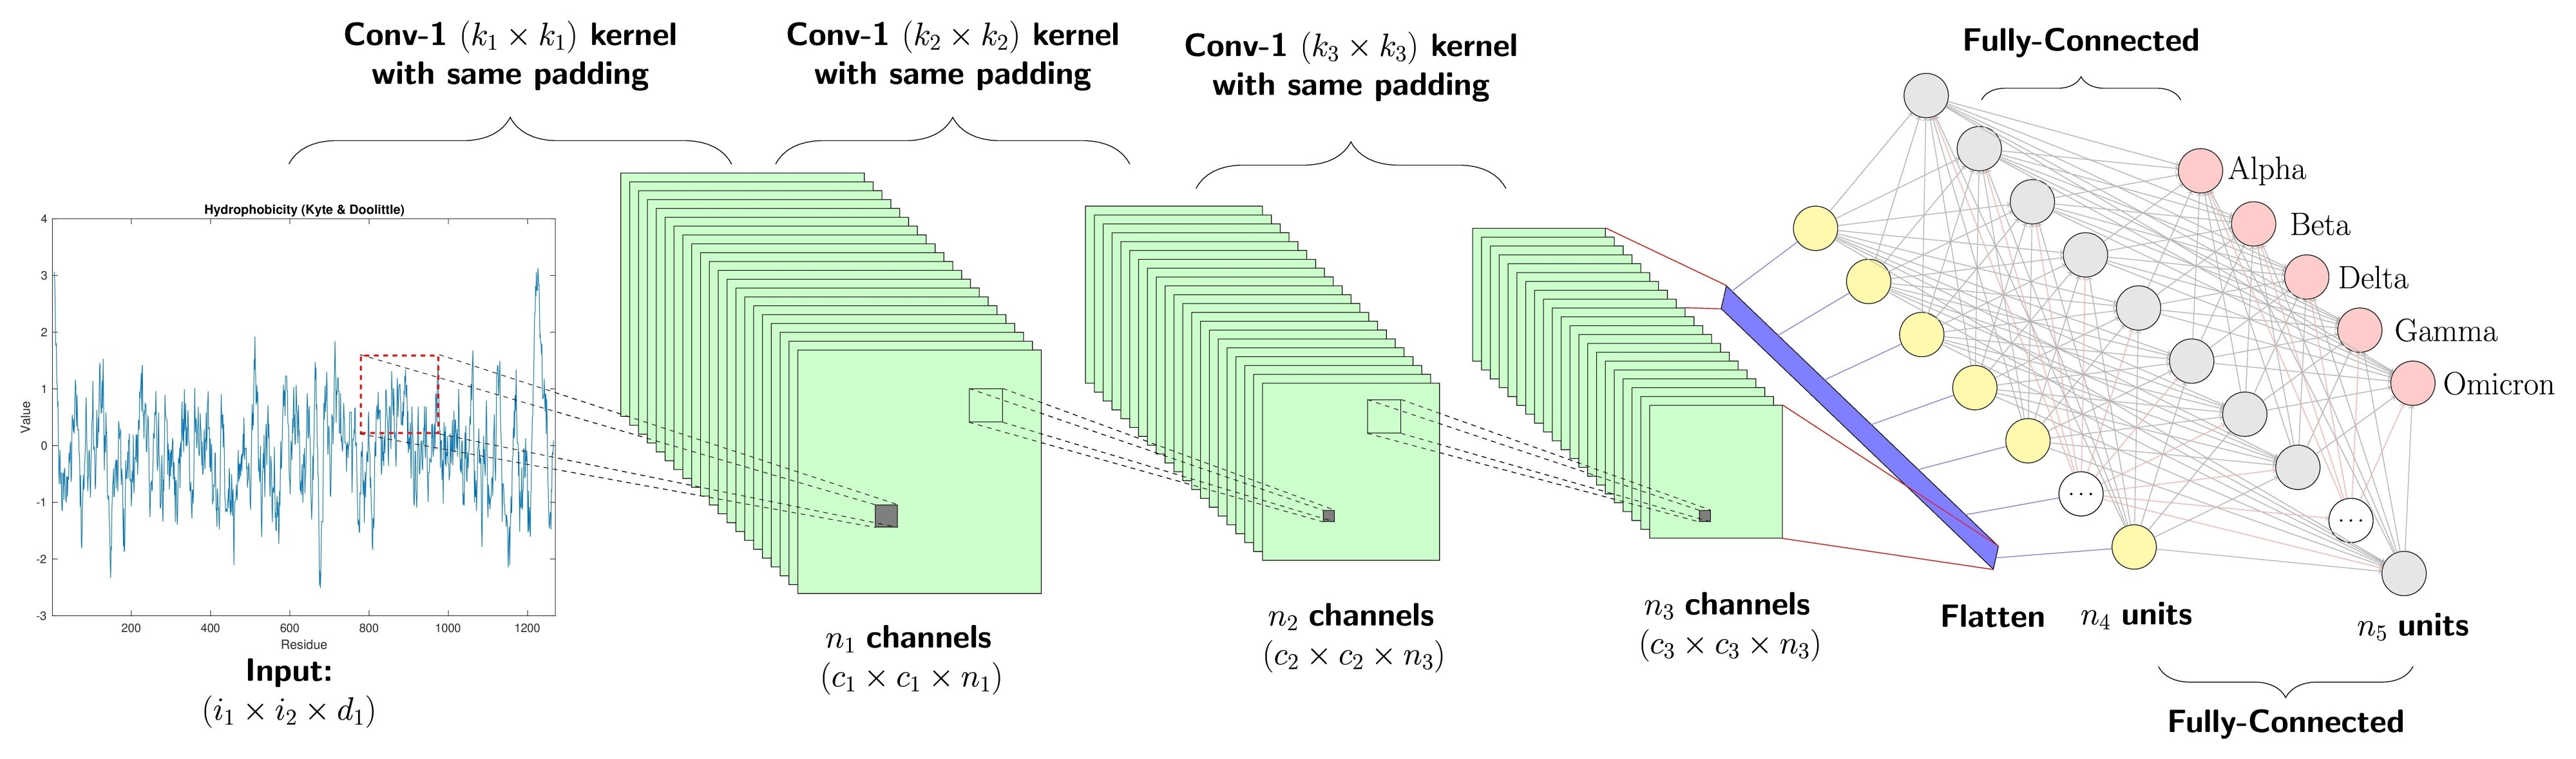
\includegraphics[width=0.8\textwidth]{2_2_convolution.jpeg}
    \caption{Minh họa các phép toán tích chập và gộp trong CNN.}
    \label{fig:cnn_ops}
\end{figure}

\subsubsection{Mô hình dựa trên Transformer}
Vision Transformer (ViT) chia ảnh thành các miếng vá, xử lý như chuỗi token, sử dụng cơ chế Self-Attention: $\text{Attention}(Q, K, V) = \text{softmax}\left(\frac{QK^T}{\sqrt{d_k}}\right)V$, với $Q, K, V$ là ma trận Query, Key, Value.\autocite{dosovitskiy2021} ViT vượt qua giới hạn cục bộ của CNN bằng cách học mối quan hệ toàn cục.

\begin{figure}[h]
    \centering
    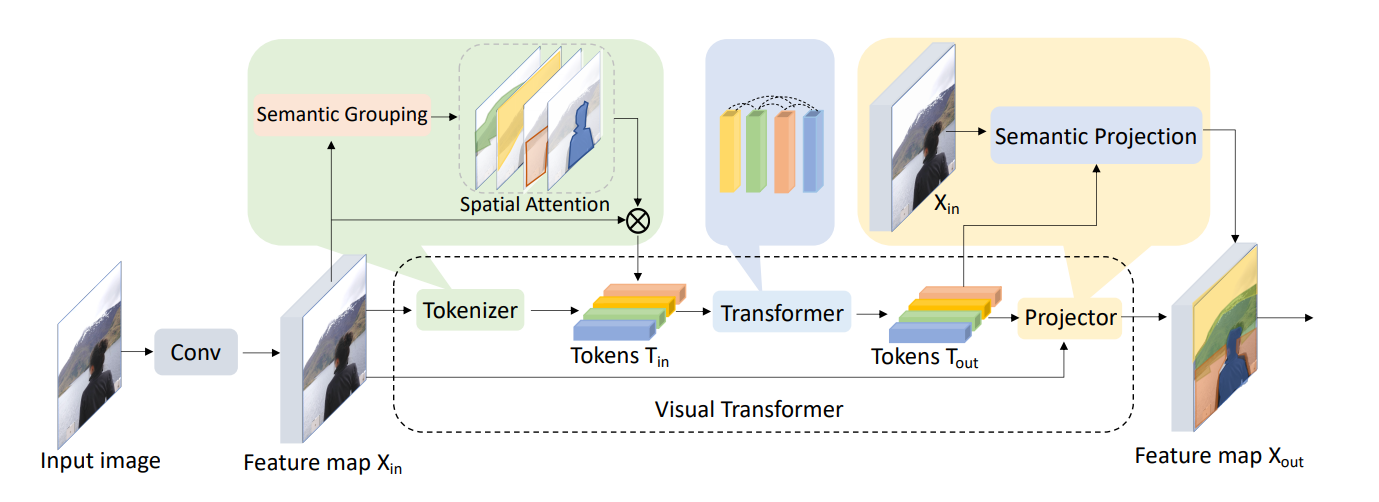
\includegraphics[width=0.9\textwidth]{visual_transformer.png}
    \caption{Kiến trúc Vision Transformer chuyển đổi hình ảnh thành chuỗi token.}
    \label{fig:vit_arch}
\end{figure}

\subsubsection{Mô hình Phân tích Cấp cao}
U-Net dùng encoder-decoder cho phân đoạn pixel-wise.\autocite{ronneberger2015} Optical flow (Horn-Schunck) tính chuyển động: $I_x u + I_y v + I_t = 0$.\autocite{horn1981} Quyết định dựa trên SVM hoặc ngưỡng trên đặc trưng.\autocite{szeliski2010}

\subsection{Các tập dữ liệu phổ biến và thước đo đánh giá mô hình}
\begin{itemize}
    \item \textbf{Tập dữ liệu}:
    \begin{itemize}
        \item ImageNet: Hơn 14 triệu ảnh, 20,000 lớp.\autocite{deng2009}
        \item COCO: Phát hiện và phân đoạn đối tượng.\autocite{lin2014}
        \item MPII, COCO Keypoints: Ước lượng tư thế người.\autocite{lin2014}
    \end{itemize}
    \item \textbf{Metrics}:
    \begin{itemize}
        \item IoU: $\frac{\text{Area of Overlap}}{\text{Area of Union}}$.\autocite{lin2014}
        \item mAP: Trung bình Average Precision trên các lớp.\autocite{lin2014}
        \item F1-score: Trung bình điều hòa Precision và Recall.\autocite{szeliski2010}
        \item OKS: Đo lường độ chính xác khớp trong HPE.\autocite{lin2014}
    \end{itemize}
\end{itemize}

Ví dụ thực tế: Hệ thống tự lái dùng CNN để nhận diện làn đường từ cạnh và gradient, kết hợp optical flow để dự đoán chuyển động.\autocite{redmon2016}

\section{Nhận diện Tư thế Người và Phát hiện Té ngã}
\label{sec:pose_fall_system}

Mục này trình bày tổng quan về nhận diện tư thế người (Human Pose Estimation - HPE), giải pháp thời gian thực MediaPipe Pose, xây dựng thuật toán phát hiện té ngã dựa trên đặc trưng động học (kinematic) và tư thế (postural), cùng mô tả chi tiết hệ thống tích hợp.

\subsection{Nhận diện Tư thế Người (Human Pose Estimation)}

Nhận diện tư thế người là một lĩnh vực then chốt trong thị giác máy tính, nhằm xác định vị trí và hướng các khớp (joints) và bộ phận cơ thể từ hình ảnh hoặc chuỗi video. Khả năng này là nền tảng cho các ứng dụng giám sát an toàn, phân tích chuyển động, và nhận diện hành vi bất thường (như té ngã).

\subsubsection{Khái niệm và Định nghĩa}

Pose Estimation ước lượng vị trí của các bộ phận cơ thể trong không gian 2D hoặc 3D, được biểu diễn qua tập hợp các \textbf{keypoints} (khớp/điểm mốc):
\begin{equation}
\mathcal{K} = \{k_1, k_2, ..., k_n\}, \quad k_i = (x_i, y_i, z_i, c_i)
\end{equation}
trong đó $(x_i, y_i, z_i)$ là tọa độ không gian (với $z_i$ là tọa độ chiều sâu tương đối) và $c_i$ là độ tin cậy (\textbf{confidence score}) của keypoint thứ $i$.

\paragraph{Phân loại Phương pháp HPE:}
\begin{itemize}
    \item \textbf{Top-down Approach:} Đầu tiên phát hiện đối tượng người, sau đó ước lượng keypoints cho từng hộp giới hạn (bounding box) của người. (VD: Mask R-CNN, MediaPipe).
    \item \textbf{Bottom-up Approach:} Đầu tiên phát hiện tất cả các keypoints, sau đó nhóm chúng lại để tạo thành tư thế của từng người. (VD: OpenPose).
\end{itemize}

%%%%%%%%%%%%%%%%%%%%%%%%%%%%%%%%%%%%%%%%%%%%%%%%%%%%%%%%%%%%%%%%%%%%%%%%%%%%%%%%
\subsection{MediaPipe Pose Estimation cho Ứng dụng Thời gian thực}

MediaPipe Pose, dựa trên mô hình **BlazePose** của Google, được tối ưu hóa để cung cấp giải pháp HPE 3D nhanh và chính xác trong môi trường thời gian thực trên nhiều nền tảng (Mobile, Web, Desktop).

\subsubsection{Kiến trúc xử lý Graph-based}

MediaPipe sử dụng kiến trúc xử lý dữ liệu dựa trên đồ thị (Graph-based Processing), nơi các nhiệm vụ được tổ chức thành một chuỗi các module:
\begin{itemize}
    \item \textbf{Nodes (Calculator):} Các module xử lý độc lập thực hiện các nhiệm vụ cụ thể (VD: Phát hiện đối tượng, Ước lượng điểm mốc).
    \item \textbf{Edges (Packet Stream):} Các luồng dữ liệu (packets) được truyền tải giữa các Nodes, đảm bảo đồng bộ hóa và nhất quán dữ liệu giữa các bước.
\end{itemize}

\subsubsection{Các thành phần Mô hình Chính}

\paragraph{Pose Detection Model (Localization):} Nhiệm vụ là phát hiện sự hiện diện và xác định \textbf{Vùng quan tâm (ROI)} chứa người trong khung hình.
\begin{itemize}
    \item Input: Khung hình RGB.
    \item Output: Bounding box và xác suất hiện diện của người.
\end{itemize}

\paragraph{Pose Landmark Model (BlazePose):} Mô hình ước lượng các điểm mốc chính xác trên ROI đã xác định.
\begin{itemize}
    \item Output: 33 keypoints 3D $(x, y, z, visibility)$.
    \item Hàm mất mát (\textbf{Loss Function}) tổng hợp:
    \begin{equation}
    \mathcal{L}_{\text{total}} = \lambda_1 \mathcal{L}_{\text{coord}} + \lambda_2 \mathcal{L}_{\text{confidence}} + \lambda_3 \mathcal{L}_{\text{depth}}
    \end{equation}
\end{itemize}

\paragraph{Pose Tracking Model:} Dự đoán ROI cho khung hình tiếp theo dựa trên pose hiện tại. Việc này giúp giảm đáng kể chi phí tính toán (computational cost) bằng cách tránh chạy mô hình phát hiện đầy đủ ở mỗi khung hình.

\subsubsection{Thuật toán Hậu xử lý (Post-processing)}

\paragraph{Temporal Smoothing (One Euro Filter):} Áp dụng bộ lọc thời gian để làm mịn tín hiệu tọa độ keypoint qua các khung hình, loại bỏ nhiễu và tăng độ ổn định của chuyển động ước tính.

\paragraph{3D Coordinate Estimation:} Chiều sâu tương đối $z$ được chuẩn hóa dựa trên kích thước cơ thể (thường là khoảng cách giữa hông).

%%%%%%%%%%%%%%%%%%%%%%%%%%%%%%%%%%%%%%%%%%%%%%%%%%%%%%%%%%%%%%%%%%%%%%%%%%%%%%%%
\subsection{Thuật toán Phát hiện Té ngã Multi-stage}

Hệ thống phát hiện té ngã sử dụng các đặc trưng động học (Kinematic) và tư thế (Postural) được trích xuất từ dữ liệu keypoints 3D (từ MediaPipe) để đưa ra quyết định qua nhiều giai đoạn. $\Delta t$ được định nghĩa là thời gian trôi qua giữa hai khung hình liên tiếp ($1/FPS$).

\subsubsection{Trích xuất Đặc trưng Sinh học (Feature Engineering)}

\paragraph{Kinematic Features (Đặc trưng Động học):} Phản ánh tốc độ và gia tốc trong quá trình té ngã.
\begin{itemize}
    \item \textbf{Vận tốc COM ($\vec{v}_{\text{COM}}$) và Gia tốc COM ($a_{\text{total}}$):}
    \begin{align}
    \vec{v}_{\text{COM}}(t) &= \frac{\vec{p}_{\text{COM}}(t) - \vec{p}_{\text{COM}}(t-\Delta t)}{\Delta t} \\
    \vec{p}_{\text{COM}} &= \frac{\sum_i w_i \vec{p}_i c_i}{\sum_i w_i c_i} \quad (\text{Với } w_i \text{ là trọng số khối lượng sinh học}) \\
    a_{\text{total}}(t) &= \frac{\|\vec{v}_{\text{COM}}(t) - \vec{v}_{\text{COM}}(t-\Delta t)\|}{\Delta t}
    \end{align}
\end{itemize}

\paragraph{Postural Features (Đặc trưng Tư thế):} Phản ánh hình dạng cơ thể và độ cao sau khi té ngã.
\begin{itemize}
    \item \textbf{Tỷ lệ Khía cạnh (Aspect Ratio - AR):} Tỷ lệ giữa chiều rộng và chiều cao của hộp giới hạn người, tăng vọt khi người nằm ngang.
    \item \textbf{Góc Nghiêng Cơ thể ($\theta_{\text{body}}$):} Góc tạo bởi trục cơ thể (vai-hông) so với phương thẳng đứng.
    \item \textbf{Độ giảm chiều cao ($\Delta h_{\text{head}}$):} Sự thay đổi vị trí của đầu so với trạng thái ban đầu.
\end{itemize}

\subsubsection{Thuật toán Phát hiện Té ngã Ba Giai đoạn}

\paragraph{Stage 1: Pre-fall Detection (Phát hiện Sớm)}
Kiểm tra các dấu hiệu ban đầu của sự mất kiểm soát, chủ yếu dựa vào tốc độ và gia tốc của Trung tâm Khối lượng (COM).

\paragraph{Stage 2: Fall Event Verification (Xác nhận Sự kiện Té ngã)}
Nếu Stage 1 là True, kiểm tra các đặc trưng tư thế (AR, $\theta_{\text{body}}$) để xác nhận trạng thái cơ thể chuyển từ đứng/đi sang nằm ngang.

\paragraph{Stage 3: Post-fall Inactivity Check (Kiểm tra Bất động sau té ngã)}
Sau khi té ngã được xác nhận (Stage 2 là True), hệ thống theo dõi mức độ chuyển động trong một khoảng thời gian ($T_{\text{window}}$). Nếu sự chuyển động thấp hơn ngưỡng $M_{th}$ trong thời gian dài, cảnh báo được kích hoạt, loại trừ các trường hợp ngồi hoặc nằm chủ động.

\subsection{Triển khai và Tối ưu hóa Hệ thống Tích hợp}

\subsubsection{Chuỗi Xử lý Dữ liệu (Data Flow Pipeline)}
Hệ thống được thiết kế theo kiến trúc module để dễ dàng tích hợp và tối ưu hóa hiệu suất:
\begin{equation}
\text{Video Stream} \xrightarrow{\text{MediaPipe}} \text{Keypoints} 
\xrightarrow[\text{Kinematic/Postural}]{3\text{D/Temporal Filtering}} \text{Feature Extraction} 
\xrightarrow{\text{Multi-stage Logic}} \text{Decision Engine} 
\xrightarrow{\text{Alert System}} \text{Response}
\end{equation}

\subsubsection{Tối ưu hóa Tham số (Parameter Tuning)}
Việc điều chỉnh các ngưỡng ($V_{th}, A_{th}, AR_{th}, \dots$) là rất quan trọng. Việc sử dụng \textbf{Ngưỡng Thích ứng (Adaptive Thresholds)} $V_{th}^{adaptive}(t)$ (phụ thuộc vào độ tin cậy của keypoints $c_i$) có thể cải thiện độ chính xác trong các môi trường nhiễu hoặc ánh sáng yếu.

\section{Cơ sở Lý thuyết về Phần cứng và Kiến trúc Hệ thống Phát hiện Té ngã}
\label{sec:hardware_theory}

Mục này cung cấp kiến thức nền tảng về phần cứng, các loại cảm biến và module truyền thông được sử dụng trong hệ thống phát hiện té ngã.

\subsection{Tổng quan Kiến trúc Hệ thống Phát hiện Té ngã}
Hệ thống phát hiện té ngã hiện đại thường được phân loại thành hai nhóm chính: \textbf{Hệ thống dựa trên Camera} và \textbf{Hệ thống dựa trên Thiết bị đeo}. Báo cáo này tích hợp cả hai, bao gồm các thành phần cốt lõi:
\begin{enumerate}
    \item \textbf{Thiết bị Thu thập Dữ liệu}: Thu thập dữ liệu chuyển động (IMU) và/hoặc hình ảnh (Camera).
    \item \textbf{Máy chủ Xử lý}: Thực hiện các thuật toán học sâu và logic ra quyết định phức tạp.
    \item \textbf{Hệ thống Truyền thông}: Đảm bảo luồng dữ liệu hai chiều và kích hoạt cảnh báo.
\end{enumerate}

\subsection{Cảm biến và Xử lý Dữ liệu Sơ cấp tại biên}

\subsubsection{Vi điều khiển và Xử lý Cục bộ}
\textbf{ESP32 (hoặc ESP32-S3)} được chọn làm bộ điều khiển trung tâm nhờ kiến trúc \textbf{lõi kép Xtensa LX6} (hoặc S3), cho phép xử lý song song. Một lõi được dành riêng cho các tác vụ thời gian thực như đọc và tiền xử lý dữ liệu cảm biến (ví dụ: \textbf{Kalman Filter} để ước tính hướng và trạng thái), trong khi lõi còn lại quản lý các giao tiếp không dây (Wi-Fi, Bluetooth) và giao thức \textbf{MQTT} hoặc \textbf{HTTP}, giảm thiểu độ trễ.

\subsubsection{Cảm biến Đo lường Quán tính (IMU)}
\textbf{IMU (Inertial Measurement Unit)} là thành phần chính trong hệ thống đeo người, cung cấp dữ liệu về động học của cơ thể. IMU tích hợp:
\begin{itemize}
    \item \textbf{Gia tốc kế}: Đo gia tốc tuyến tính. Gia tốc thô được hiệu chuẩn để chuyển từ giá trị số nguyên sang đơn vị thực tế ($g$).
    \item \textbf{Con quay hồi chuyển}: Đo tốc độ góc, dựa trên \textbf{hiệu ứng Coriolis}.
    \item \textbf{Từ kế}: Cung cấp tham chiếu hướng từ trường để hiệu chỉnh sai số trôi của con quay hồi chuyển (thường thông qua thuật toán \textbf{Sensor Fusion} như Bộ lọc Madgwick hoặc Kalman).
\end{itemize}

Dữ liệu thô sau khi xử lý (ví dụ: trung bình hóa) được biểu diễn dưới dạng vector 3D:
\[
\mathbf{a} = [a_x, a_y, a_z], \quad
\boldsymbol{\omega} = [\omega_x, \omega_y, \omega_z]
\]

\paragraph{Phát hiện Té ngã dựa trên Ngưỡng IMU}
Tại tầng vi điều khiển, té ngã được phát hiện sơ bộ bằng cách phân tích sự thay đổi đột ngột của \textbf{Gia tốc Tổng (Magnitude of Acceleration)} và tốc độ góc:
\begin{itemize}
    \item \textbf{Shock Event}: Gia tốc tổng vượt ngưỡng cao ($a_{\text{shock}}$): $\|\mathbf{a}\| > a_{\text{shock}}$.
    \item \textbf{Post-fall State}: Gia tốc tổng sau đó giảm về gần 1g (biểu thị trạng thái nằm ngang) trong khi tốc độ góc có thay đổi lớn.
\end{itemize}
\[
\|\mathbf{a}\| = \sqrt{a_x^2 + a_y^2 + a_z^2}
\]

\subsubsection{Cảm biến Định vị Vị trí (GPS)}
Module GPS (ví dụ: u-blox NEO-6M) sử dụng nguyên lý \textbf{Đo tam giác} để xác định vị trí địa lý của thiết bị dựa trên tín hiệu từ ít nhất bốn vệ tinh. Dữ liệu đầu ra là chuỗi \textbf{NMEA}, cung cấp tọa độ Kinh độ/Vĩ độ và độ cao, là thông tin quan trọng cho dịch vụ cứu hộ khẩn cấp.

\subsection{Hệ thống Camera và Xử lý Máy chủ}

\subsubsection{Hệ thống Camera}
Camera nhúng (\textbf{ESP32-S3 + OV5640 5MP}) cung cấp dữ liệu hình ảnh được nén theo chuẩn \textbf{JPEG}. Dữ liệu này là luồng byte được truyền tải qua Wi-Fi bằng các giao thức như \textbf{RTSP} hoặc \textbf{HTTP/MJPEG stream}, phục vụ cho việc \textbf{Xác minh Hình ảnh} trên máy chủ.

\subsubsection{Kiến trúc Máy chủ Xử lý}
Máy chủ là nơi thực hiện các thuật toán phức tạp như Ước lượng tư thế người (HPE) và Học sâu, đảm bảo độ chính xác cao.
\begin{itemize}
    \item \textbf{Phần cứng}: Sử dụng máy chủ đám mây (AWS, Google Cloud) hoặc máy tính nhúng mạnh mẽ (NVIDIA Jetson Nano) có \textbf{GPU} để tăng tốc tính toán Tensor.
    \item \textbf{Phần mềm Học sâu}: Nền tảng \textbf{TensorFlow/PyTorch} kết hợp với thư viện \textbf{OpenCV}.
    \item \textbf{Xử lý Dữ liệu Lớn}: Máy chủ tiếp nhận luồng dữ liệu \textbf{JSON/MQTT} (từ IMU) và luồng \textbf{JPEG} (từ Camera). Việc tổng hợp và đồng bộ hóa hai luồng dữ liệu này là chìa khóa để xác minh té ngã và giảm thiểu báo động giả (False Positives).
\end{itemize}

\subsection{Hệ thống Truyền thông và Cơ chế Dự phòng}

\subsubsection{Module Truyền thông Đa dạng}
\begin{itemize}
    \item \textbf{Wi-Fi (ESP32)}: Kênh chính để truyền tải dữ liệu dung lượng lớn (video/hình ảnh) và giao tiếp \textbf{MQTT} với máy chủ.
    \item \textbf{Module Di động (4G/LTE - EC800K)}: Đóng vai trò là \textbf{Kênh Dự phòng}. Nó hỗ trợ định vị GPS và quan trọng nhất là kích hoạt \textbf{cuộc gọi khẩn cấp tự động} hoặc gửi \textbf{SMS cảnh báo} bằng \textbf{AT commands}, đảm bảo cảnh báo được gửi đi ngay cả khi mạng Wi-Fi không khả dụng.
\end{itemize}

\subsubsection{Liên kết Tổng thể và Logic Dự phòng}
Hệ thống vận hành theo nguyên lý tích hợp và dự phòng:
\begin{enumerate}
    \item \textbf{Thu thập/Xử lý Sơ cấp}: ESP32 thu thập IMU/Camera và thực hiện phát hiện té ngã dựa trên ngưỡng IMU.
    \item \textbf{Quyết định Truyền thông}: Nếu té ngã được phát hiện, dữ liệu được truyền đến máy chủ qua kênh Wi-Fi (Ưu tiên) hoặc 4G (Dự phòng).
    \item \textbf{Xác minh Máy chủ}: Máy chủ tiến hành phân tích hình ảnh (HPE) kết hợp với dữ liệu IMU để xác minh té ngã (Multi-stage Fall Detection Logic).
    \item \textbf{Kích hoạt Cảnh báo}: Nếu xác nhận té ngã, máy chủ ra lệnh cho ESP32 kích hoạt Module EC800K gửi cảnh báo (SMS/Cuộc gọi), hoàn tất chu trình cứu hộ.
\end{enumerate}

\subsubsection{Môi trường Phát triển Phần mềm Nhúng}
Việc phát triển phần mềm cho các vi điều khiển như ESP32 đòi hỏi một framework chuyên biệt. \textbf{ESP-IDF (Espressif IoT Development Framework)} được chọn làm môi trường phát triển chính thay vì các IDE đơn giản hơn (như Arduino IDE) vì những lý do sau:
\begin{itemize}
    \item \textbf{Hỗ trợ RTOS}: ESP-IDF tích hợp \textbf{FreeRTOS}, cho phép tận dụng tối đa kiến trúc lõi kép của ESP32 để thực hiện đa nhiệm (ví dụ: một tác vụ xử lý dữ liệu IMU thời gian thực, một tác vụ quản lý kết nối Wi-Fi).
    \item \textbf{Truy cập Cấp thấp (Low-level Access)}: Cho phép truy cập trực tiếp và tối ưu hóa các thanh ghi phần cứng (Registers), cần thiết cho việc cấu hình cảm biến IMU (I2C/SPI) và tinh chỉnh các giao thức mạng phức tạp (MQTT/HTTP) ở mức độ chi tiết cao, đảm bảo hiệu suất thời gian thực.
\end{itemize}
Việc lựa chọn môi trường này là nền tảng để xây dựng các mô-đun phần mềm chuyên biệt, sẽ được trình bày chi tiết trong Chương 3.

\subsection{Tóm tắt Chương và Cơ sở cho Triển khai đề tài}
\label{sec:chapter_conclusion}

Chương này đã thiết lập nền tảng lý thuyết toàn diện, tạo cơ sở khoa học cho việc thiết kế và triển khai hệ thống phát hiện té ngã tích hợp. Những kiến thức cốt lõi đã được trình bày bao gồm:
\begin{itemize}
    \item \textbf{Cơ sở Thị giác Máy tính:} Nắm vững kiến trúc CNN và Transformer, là nền tảng cho việc xử lý hình ảnh và nhận diện tư thế người.
    \item \textbf{Phương pháp Ước lượng Tư thế Người (HPE):} Chi tiết về MediaPipe Pose (BlazePose) như một giải pháp thời gian thực, cung cấp tọa độ 3D $\mathcal{K}$ (keypoints) làm dữ liệu đầu vào cho các thuật toán phân tích hành vi.
    \item \textbf{Phần cứng Hệ thống Nhúng:} Phân tích vai trò của ESP32/ESP32-S3, cảm biến IMU (Gia tốc, Con quay, Từ kế) và Module Truyền thông (Wi-Fi, 4G), cùng với các nguyên lý xử lý tín hiệu sơ cấp như tính toán Gia tốc Tổng.
\end{itemize}

Tất cả các thành phần lý thuyết này sẽ được tích hợp trong Chương tiếp theo. Cụ thể, mô hình lý thuyết về các \textbf{đặc trưng động học} và \textbf{tư thế} (Kinematic \& Postural Features) sẽ được chuyển hóa thành các mô-đun phần mềm trên nền tảng ESP-IDF và các Framework. Chương tiếp theo, \textbf{Thiết kế và Phương pháp luận Triển khai}, sẽ tập trung vào việc kiến trúc hóa hệ thống, chi tiết hóa cấu trúc mã nguồn, và mô tả quy trình thực nghiệm được tiến hành để biến các nguyên lý cơ sở thành một giải pháp phát hiện té ngã thời gian thực, đáng tin cậy.

